% LNCS single-column build (generated from plan/sections/*.tex)
\documentclass[runningheads,a4paper]{llncs}

\usepackage[T1]{fontenc}
\usepackage{amsmath,amssymb}
\usepackage{booktabs}
\usepackage{graphicx}
\usepackage{array}
\usepackage{multirow}
\usepackage{url}
\usepackage{algorithm}
\usepackage{algpseudocode}
\usepackage{enumitem}

\graphicspath{{../../figures/}}

% Wide two-column-master figures are scaled to the LNCS text width here.
\newcommand{\dblfig}[3]{%
  \begin{figure}[!tb]\centering
    \includegraphics[width=\textwidth]{#1}%
    \caption{#2}\label{#3}
  \end{figure}}
\newcommand{\onefig}[4]{%
  \begin{figure}[!t]\centering
    \includegraphics[width=\textwidth]{#1}%
    \caption{#2}\label{#3}\vspace{#4}
  \end{figure}}

\begin{document}
\sloppy

\title{The First Round Is a Two-Sided Window: Threshold Timing and
Conditional Decoding Failure in QC-MDPC Bit-Flipping}
\titlerunning{The First Round Is a Two-Sided Window}

\author{[Author names and affiliations to be completed before submission]}
\authorrunning{[Author names to be completed]}
\institute{[Affiliations and e-mail to be completed before submission]}

\maketitle

\begin{abstract}
BIKE and other QC-MDPC designs rest on a decoding failure rate near $2^{-128}$ that no simulation can measure, and on decoder behaviour that must hold across keys that cannot be inspected. This paper measures how far a BF decoder's threshold schedule controls conditional failure. We decode paired instances: two schedules process the same key, error and syndrome, and we resample keys rather than errors when we quote uncertainty. The first round of the CLASSIC BF decoder is a sharp, asymmetric two-sided window. Raising its threshold by one to three lowers the conditional failure rate 2.3--5.5-fold across three formal conditions; lowering it by one worsens the rate about eightfold, and by two by more than two orders of magnitude. The round and persistence of the offset matter as much as its size: the same offset confined to its own round helps, while sustained through later rounds it raises the failure rate to about 4--6\% even when round one is untouched. First-round records explain the asymmetry: incorrect first-round flips fall far more than correct ones, so the intervention removes wrong decisions rather than accelerating correction. The effect transfers to a second operating point and a larger code without retuning, and stops at the tested capture-prone constructions. At the production block size it reproduces once the error weight is raised; at the production weight only a decision margin and a convergence cost are measurable. A round-one surrogate did not predict the effect of another schedule, and the failure is diagnosed.
\keywords{post-quantum cryptography \and QC-MDPC codes \and bit-flipping
decoding \and decoding failure rate \and first-round threshold \and
key-conditional risk.}
\end{abstract}

\section{Introduction}\label{sec:intro}

BIKE and other QC-MDPC designs rest on iterative bit-flipping (BF) decoding, whose rare failures shape their security arguments~\cite{misoczki2013mdpc,bike2024spec,alagic2025nist}. The Level-1 target is a decoding failure rate (DFR) near $2^{-128}$, far below direct simulation~\cite{sendrier2019dfr,vasseur2021thesis}. Failures are not spread evenly: they cluster on particular keys~\cite{guo2016key,wang2023weak,nosouhi2023weakkey}, and an adversary who can detect or time them recovers the key~\cite{eaton2018timing}. A decoder's per-round thresholds form a schedule that can be retuned without touching key generation. We therefore test whether a deliberate change of schedule alters failure risk for a given key.

While characterising the CLASSIC BF decoder of Vasseur's reference implementation~\cite{vasseur2021thesis}, which we denote C0, we noticed that its earliest decision is unusually delicate. Round one acts on the untouched syndrome, so a mistake there enters the state of every later round. Raising the round-one threshold by two lowers the conditional failure rate by 4.15 in the random condition and 5.47 under an adversarial probe; lowering it by one raises the rate about eightfold. A two-unit offset is also destructive when sustained from round two onward, yet helpful when confined to one round.

We rebuilt the experiment around paired instances. An instance is a key $H$, an error $e$ and its syndrome $s=He^{\top}$; every schedule variant decodes the same triple. FRO-$k$ raises the round-one threshold by $k$ in round one only, and FRONEG lowers it by one. We summarise comparisons by the risk ratio (RR), the baseline failure rate divided by the variant's, so values above one favour the variant. Because failures concentrate on keys, intervals and tests resample keys, not errors. All quoted rates lie where failures are frequent enough to count; we make no claim about the production tail.

The study has four contributions. First, the first round is a two-sided window. Conservative offsets of $+1$ to $+3$ lower the failure rate 2.3--5.5-fold, while the permissive side collapses within two counts (Section~\ref{sec:formal}). Second, the same offset changes sign with its round and persistence. The $+2$ applied once in round two gives a small benefit, but sustained from round two onward it gives RR 0.0168 (Section~\ref{sec:temporal}). Third, the mechanism is asymmetric. FRO-2 reduces incorrect first-round flips about tenfold while correct flips fall far less (Section~\ref{sec:mechanism}). Fourth, the window reproduces at the production block size once the error weight is raised, while at the production weight only a decision margin and a convergence cost are measurable (Section~\ref{sec:production}). A designed negative closes the list: a round-one surrogate did not predict the effect of another schedule (Section~\ref{sec:counterfactual}).

Section~\ref{sec:background} sets up QC-MDPC BF decoding, related work, and a first-order model of the round-one window. Section~\ref{sec:method} gives the paired design, and Section~\ref{sec:results} the results. Section~\ref{sec:discussion} interprets them and states their limits; Section~\ref{sec:conclusion} concludes.
\section{Background and related work}\label{sec:background}

This section fixes the code, the decoder, the prior work we position against, and a first-order model of the round-one window.

\subsection{QC-MDPC codes and the BF decoder}

Quasi-cyclic moderate-density parity-check (QC-MDPC) codes are binary linear codes with block-circulant parity checks \cite{misoczki2013mdpc}. We write $r$ for the block size and $n=2r$ for the code length. The parity-check matrix is $H=[H_0\mid H_1]$, where each circulant block has row weight $d$; the full matrix has row weight $2d$ and column weight $d$. The symbol $t$ is the number of errors injected into one decoding attempt. The primary operating point is $(r,d,t)=(4801,45,92)$ (Section~\ref{sec:method}). For a parity-check matrix $H$ and an error vector $e$, the syndrome is $s=He^{\top}$. A decoding attempt succeeds when the final syndrome is zero and fails otherwise.

BF decoding repairs errors iteratively. The decision variable of a position is its unsatisfied parity-check counter (UPC), the number of unsatisfied equations that involve it. In every round the decoder flips all positions whose UPC passes a threshold, recomputes the syndrome, and repeats until the syndrome vanishes or the iteration budget ends. Algorithm~\ref{alg:bf} states the procedure.

\begin{algorithm}[t]
\caption{Plain BF decoding}
\label{alg:bf}
\begin{algorithmic}[1]
\Require $H$, input syndrome $s_{\mathrm{in}}=He^{\top}$, budget $I$
\Ensure error estimate $\hat e$, or failure
\State $\hat e \gets \mathbf{0}$; $s_{\mathrm{res}} \gets s_{\mathrm{in}}$
\For{$i=1$ to $I$}
  \State compute $U_j=\mathrm{UPC}(H,s_{\mathrm{res}},\hat e,j)$ for every position $j$
  \State set $\tau_i$ from the current syndrome weight $|s_{\mathrm{res}}|$
  \State flip every $j$ with $U_j\ge\tau_i$
  \State update $\hat e$ and $s_{\mathrm{res}}\gets s_{\mathrm{in}}\oplus H\hat e^{\top}$
  \If{$s_{\mathrm{res}}=\mathbf{0}$}
    \State \textbf{return} $\hat e$
  \EndIf
\EndFor
\State \textbf{return} failure
\end{algorithmic}
\end{algorithm}

The baseline is the CLASSIC BF decoder of Vasseur's reference implementation \cite{vasseur2021thesis}, denoted C0. Its threshold is the binomial-model value of \path{compute_threshold}, rounded up and clipped to $[(d+1)/2,d]$, and recomputed from the current syndrome weight in every round. The main experiment uses a 20-round budget and static-distance semantics. Static runs use a fixed initial $t$; the offset is added to the clipped base threshold and the result is clipped again to the same interval. The archived note \path{reference/FROZEN_REFERENCE_SEMANTICS.md} shipped with the code gives the exact formula and source identity. A run stops on zero syndrome or budget exhaustion. A separately coded dynamic-distance reference uses the current distance to the true error, information a deployer does not have, and serves only as a simulation-privileged directional check. Its named descendants modify the schedule or carry additional state: Black-Gray-Flip (BGF), Backflip, and the specification's decoder, which we call BIKE-Flip \cite{drucker2020shades,vasseur2021thesis,bike2024spec}. We treat them as separate decoders. BIKE-Flip protects every round with a floor, $T=\max(f_t(S),T_i(S_0))$ \cite{bike2024spec}, where $S$ is the current syndrome weight, $f_t(S)$ an affine function of it, and $T_i(S_0)$ a floor computed from the initial syndrome weight $S_0$. Each floor equals the un-margined level plus a margin $\Delta$, so the margin persists in every iteration rather than appearing only in the first. At Level 1 the specification sets $\Delta=3$ and a budget of seven iterations. Appendix A.2.4 derives the affine constants as the tangent of the theoretical threshold at the average syndrome weight; we verified our implementation against the constants printed for Levels 1, 3 and 5. The published rationale places the residual failures at iterations two and three, where the falling syndrome weight pushes the threshold below the counters of a few correct positions \cite{sendrier2024seminar,wang2023weak}. FRO-2 takes a different route: it adds $+2$ to the round-one threshold once, and later rounds keep the plain threshold.

\subsection{Failure is conditional on keys and schedules}

Failure is conditional on the key as well as the channel. Guo et al.\ showed that error patterns triggering failure correlate with the secret matrix, so observed failures leak key information \cite{guo2016key}; Wang et al.\ turned the same correlation into a weak-key construction \cite{wang2023weak}; and Eaton et al.\ converted timing observations into a key-recovery attack \cite{eaton2018timing}. Gellersen et al.\ extended the side-channel route \cite{gellersen2025}. Weak-key classes with elevated failure rates have also been constructed, enumerated and filtered \cite{vasseur2021thesis,nosouhi2023weakkey,matthews2025combinatorial}. The schedule is a second conditioning variable, because the flips of one round shape the state entering the next. Our design therefore perturbs the schedule and treats the key as the unit of inference: all variants decode identical $(H,e,s)$ instances, and uncertainty comes from resampling keys rather than errors (Section~\ref{sec:method}).

\subsection{Related work}

Failure modelling has followed two routes. The first explains failure from decoder state. Kim and Park fit a per-instance logistic predictor \cite{kim2021logistic}; Paiva and Terada use the first-round residual error as a proxy \cite{paiva2022pickyfix}; Santini et al.\ and Annechini et al.\ analyse counters for regular codes \cite{santini2019conservative,annechini2024estimation}. The second estimates rates beyond simulation. Sendrier and Vasseur model BF as a Markov chain \cite{sendrier2019dfr,sendrier2020lowdfr}; Tillich derives failure-probability bounds \cite{tillich2018dfp}; Vasseur adds extrapolation with confidence intervals \cite{vasseur2021thesis}; Arpin et al.\ predict key-dependent error floors \cite{arpin2025errorfloor}; and Annechini et al.\ give a closed form with an explicit warning that proxy-based extrapolation is dangerous \cite{annechini2025closedform}.

A third line tunes thresholds directly. Kichna et al.\ use particle-swarm search at our block size, reporting mean iterations reduced from 5.36 to 3.01 at the recommended error weight, but no failure-rate measurement \cite{kichna2025pso}. Recent work changes the decoder itself: BF-Max \cite{baldelli2025bfmax}, in-place randomised flipping \cite{baldi2021inplace}, near-codeword-aware BF \cite{baldelli2026ncw}, and follow-up refinements \cite{santini2026flip}. These decoders are reference points for magnitude and cost, not objects we claim to dominate. Taken together, these lines motivate the question this paper pursues: does a small change in the round-one schedule alter conditional failure, and does the effect depend on the round and persistence? We test that question on paired instances; Section~\ref{sec:counterfactual} adds a secondary diagnostic, asking whether the same first-round statistics can predict another schedule.
\subsection{A first-order model of the first-round window}\label{sec:model}

The model is deliberately minimal. It describes how a small raise of the round-one threshold reshapes the flips of that round; later rounds are outside its scope.

Fix an instance, that is a key $H$ with an error $e$ and its syndrome $s$. In round one each position $j$ carries a counter $U_j$, its UPC. The decoder flips the positions whose counter reaches the round-one threshold $\tau_1$, and nothing else.

Error positions and clean positions look different to the decoder. A position in the error support contributes its own error to every incident check, so most of its checks are unsatisfied; a clean position's checks are unsatisfied only through other errors. Under the independence approximation used for first-iteration UPC distributions~\cite{annechini2024estimation}, the two populations follow separate binomial laws with per-check probabilities $p_1>p_0$:
\begin{equation}\label{eq:upc-tails}
\begin{aligned}
U_{i,j} &\sim \operatorname{Bin}(d,p_i), \qquad i\in\{1,0\},\; p_1>p_0,\\
q_i(\tau) &= \Pr[U_{i,j}\ge\tau]
= \textstyle\sum_{u=\tau}^{d}\binom{d}{u}p_i^{u}(1-p_i)^{d-u}.
\end{aligned}
\end{equation}
Here $i=1$ marks an error position and $i=0$ a clean one. The tail mass $q_i(\tau)$ is the probability that a class-$i$ position flips at threshold $\tau$, so $q_1$ governs true flips and $q_0$ false flips. The probabilities are model parameters, not fitted quantities; the multipliers below are computed from the archived first-round census, so the model is used qualitatively.

The perturbation is a one-shot raise $\tau_1\to\tau_1+2$. A raise acts on each population through the fraction of flips that survives it:
\begin{equation}\label{eq:multipliers}
A_1=\frac{q_1(\tau_1+2)}{q_1(\tau_1)},\qquad
A_0=\frac{q_0(\tau_1+2)}{q_0(\tau_1)} .
\end{equation}
The model predicts $A_0\ll A_1$: the clean tail at $\tau_1$ is the thinner, outer tail, so two extra counts cut into it disproportionately. At the held-out point $P_4=(3607,39,76)$ the archived profile gives $A_1 = 0.355$ and $A_0 = 0.0892$. Both lie below one, so the raise thins both populations, and the far smaller $A_0$ places the thinning mainly on false flips, the favourable direction. The deferred true flips remain the price.

Three testable consequences organise the empirical programme.
\begin{enumerate}[label=(\roman*),leftmargin=*,itemsep=1pt,topsep=2pt]
\item The round-one census should show the asymmetry directly, with false flips falling by a much larger relative factor than true flips (Section~\ref{sec:mechanism}).
\item The net failure change has no locally fixed sign, because deferred true flips are a countervailing cost; the paired window must settle it (Section~\ref{sec:results}).
\item The model constrains one round only, so a sustained offset is a distinct experiment (Section~\ref{sec:temporal}).
\end{enumerate}
The model is silent on the sign of the net failure change and on rounds after the first. Consequences (ii) and (iii) are therefore experiments rather than corollaries.
\section{Study design}\label{sec:method}

The model of Section~\ref{sec:model} is silent on the sign of the first-round window; this section fixes the protocol that measures it. The baseline is C0 and the intervention is FRO-2, both defined in Section~\ref{sec:intro}.

For each variant within each condition, we estimate the DFR as the number of failed decodings divided by the number attempted. Interval uncertainty comes from a $95\%$ bootstrap over keys rather than over error draws, so intervals reflect key-to-key variation. A zero-failure entry is never read as zero risk; the rule-of-three bound $3/N$ replaces it over $N$ attempts. Every comparison reduces to the risk ratio, C0's DFR divided by the variant's, and values above one favour the variant. Variants differ only in the threshold schedule; the iteration budget and every other setting are held fixed.

Interval and test conventions were fixed before the runs. Intervals are percentile cluster-bootstrap intervals over keys: 10{,}000 resamples per contrast, keys drawn with replacement while every error draw of a selected key is retained, with the bootstrap seed fixed at 20260905. The sign test counts the keys on which the variant fails less often than C0, drops ties, and returns an exact two-sided binomial probability. Holm correction covers the three formal conditions of the primary comparison; the temporal grid, the transfer checks and the decoder comparisons are reported as marginal intervals. All computations are reproducible from the archived per-key counts.

The study uses eight operating points, each with a role. The primary point is $P_1'=(4801,45,92)$; the prime marks the measurable variant of the screening point $P_1=(4801,45,84)$ at which candidate schedules were compared before formal measurement. The transfer points are $P_2=(3001,37,66)$ and $P_3=(4001,41,82)$, and $P_4=(3607,39,76)$ is held out for a rule check. The largest block in the series is $(6007,56,100)$. At the production block $(12323,71)$ the study measures a raised weight $(t^{\ast}=172)$ and the production weight 134; the CPA-128 preset is $(10163,71,140)$.

Three key/error sampling conditions are used throughout. RAND draws the key at random and the error uniformly at weight $t$. TYPE-I constrains one parity-check block of the key to contain a run of $12$ consecutive ones, with the error drawn as in RAND; it is an adversarial probe, not a population estimate. NCW-shallow uses a key pool filtered to admit a near-codeword pattern and builds the error with overlap $\kappa=12$, below the block row weight $d=45$. The shallow condition is a stress construction, not a proof that capture is impossible; a separate stress family that crosses $d$ appears in Section~\ref{sec:boundary}. Figure~\ref{fig:design} shows the pairing and the run streams.

The protocol ran in stages, from calibration to a single confirmation on fresh keys. We first calibrated the primary family where failures are measurable, so every compared difference sits above the zero-failure floor. Before prespecification we screened nine candidate schedules under a worst-group bound, which reads the weakest condition so a schedule cannot hide harm in one condition behind gains in another. The prespecified gate required the worst-group $95\%$ upper bound to improve by at least $0.5$ in $\log_{10}$ units (a factor of 3.2), and the primary condition had to stay non-inferior. The gate was evaluated once on a pure-fresh subset: 212 keys with 3000 draws each, 636{,}000 per variant. Those keys never entered screening, so the confirmation is independent of every selection decision; the subset remains part of the 278-key formal pool, so this independence is from the selection procedure, not a second statistically independent estimate. Four frozen master seeds govern the master, bootstrap, exploratory and confirmation streams, so every run is exactly reproducible.

Every number reported later is reproducible from the frozen exports. A second implementation, written independently within the same project, recorded 11 failures in 20{,}000 dynamic-distance decodes against 136 in 200{,}000 in the C reference ($z=-0.68$), and reproduced the direction of the primary contrast. That cross-check bounds coding error only, because both implementations share the design assumptions. An exact-recovery audit covered all 278 formal $P_1'$ keys and 834{,}000 decodings per variant. It found 795 exact-recovery failures for C0 and 167 for FRO-2, matching the zero-syndrome totals, with no miscorrection in either variant. The main experiment uses static-distance semantics while the C reference uses dynamic distances, so their rates are never compared. Exploratory entries and archived prototypes remain labelled and never carry a primary conclusion.

\dblfig{fig1_study_design.pdf}{Study design. (a)~Both schedules decode the same key, error and syndrome. (b)~FRO-2 adds two in round one only; from round two onward both use the C0 schedule. (c)~Outcomes are paired per key, and keys are the resampling unit.}{fig:design}
\section{Results}\label{sec:results}

This section reports the measured evidence in a fixed order: the window, its timing, its mechanism, its transfer, its boundaries, and the decoder reference comparison.

\subsection{The first round is a two-sided window}\label{sec:formal}

Every instance is decoded by C0 and by FRO-2, which adds $+2$ to the round-one threshold alone. Both variants see the same key, error and syndrome. The comparison runs at $P_1'=(4801,45,92)$ under RAND, TYPE-I and NCW-shallow. Table~\ref{tab:main} gives the counts and tests; Figure~\ref{fig:main} gives the absolute rates, intervals and per-key distributions.

FRO-2 lowers the failure rate in all three conditions (Table~\ref{tab:main}). The RR is 4.15 [3.29, 5.38] under RAND, 5.47 [4.25, 7.28] under TYPE-I and 4.55 [3.21, 6.82] under NCW-shallow; every interval excludes one, and the key-clustered sign test agrees after Holm correction. Per key, FRO-2 improves 233 of the 278 condition-by-key cases, worsens 18 and ties 27. The prespecified gate asked whether the worst condition's $95\%$ DFR upper bound improved by at least $0.5$ $\log_{10}$ units (a factor of 3.2). It improved by 0.679 $\log_{10}$ in the full pool (a factor of 4.8) and 0.687 in the fresh subset, so the gate passed.

The two sides of the window are unequal. FRONEG subtracts one at round one: it worsens all 92 RAND keys and lifts failures from 282 to 2{,}235, an RR of 0.126 [0.111, 0.141], a 7.93-fold rise. One step down therefore costs more than two steps up gain.

The full local scan resolves both sides (Figure~\ref{fig:window}). Offsets $+1$ to $+3$ lower the rate by about 2.3- to 5.5-fold, with the maximum at $+2$ or close to it. The permissive side collapses within two counts: one count down gives RR 0.10--0.13, and two counts down 0.0014--0.0030. Under RAND the two-count decrease multiplies failures by 365, from 282 to 102{,}980 of 276{,}000. The window is two-sided and sharply asymmetric. In plain terms, a conservative offset buys a 4--5-fold reduction, while one step down more than cancels it.

\begin{table}[!tb]
\centering
\footnotesize
\setlength{\tabcolsep}{3pt}
\caption{Primary comparison at $P_1'=(4801,45,92)$. Cells give failures/decodings and DFR. RR is C0 over FRO-2 with 95\% key-cluster bootstrap intervals; Holm $p$ is the key-clustered sign test across the three conditions.}
\label{tab:main}
\begin{tabular}{@{}lccc@{}}
\toprule
 & RAND & TYPE-I & NCW-shallow \\
\midrule
Keys & 92 & 94 & 92 \\
C0 failures/decodings & 282/276{,}000 & 372/282{,}000 & 141/276{,}000 \\
C0 DFR & $1.02\times10^{-3}$ & $1.32\times10^{-3}$ & $5.11\times10^{-4}$ \\
FRO-2 failures/decodings & 68/276{,}000 & 68/282{,}000 & 31/276{,}000 \\
FRO-2 DFR & $2.46\times10^{-4}$ & $2.41\times10^{-4}$ & $1.12\times10^{-4}$ \\
RR [95\% CI] & 4.15 [3.29, 5.38] & 5.47 [4.25, 7.28] & 4.55 [3.21, 6.82] \\
Holm $p$ & $4.88\times10^{-17}$ & $3.05\times10^{-22}$ & $7.66\times10^{-12}$ \\
\bottomrule
\end{tabular}
\end{table}


\dblfig{fig2_main_results.pdf}{Primary comparison at $P_1'=(4801,45,92)$. (a)~Absolute failures per 10{,}000 decodes. (b)~Risk ratio C0/FRO-2 with 95\% key-cluster bootstrap intervals; the dashed line marks one. (c--e)~Per-key distribution of failures avoided under RAND, TYPE-I and NCW-shallow; counts give improved, worsened and tied keys. Each key has 3{,}000 decodes per schedule.}{fig:main}

\begin{figure}[!t]
\centering
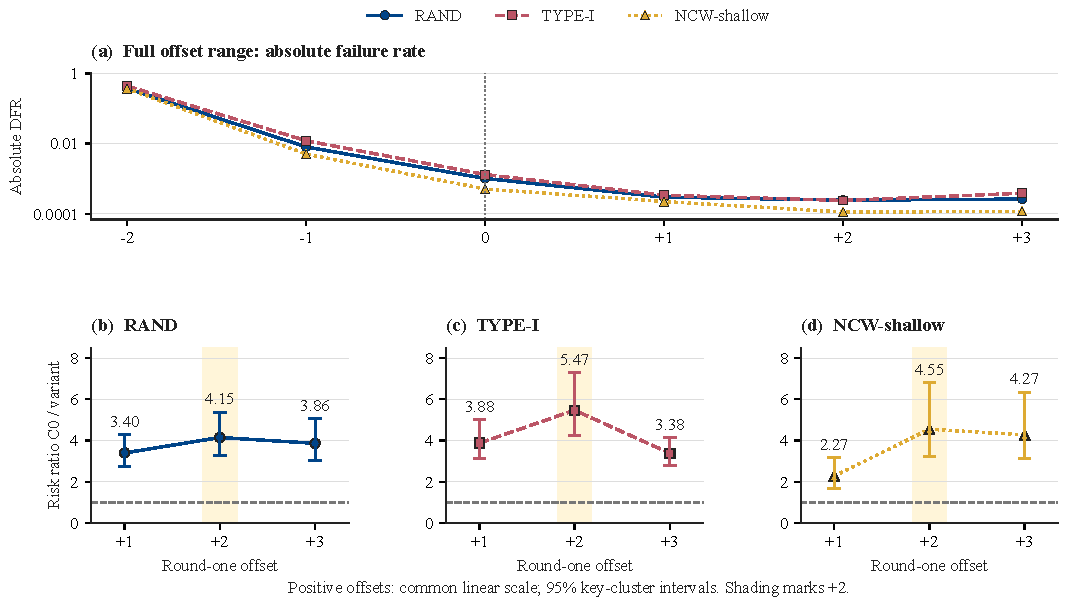
\includegraphics[width=0.94\textwidth]{fig6_threshold_window.pdf}
\caption{The first round is a two-sided window at $P_1'$. (a)~Absolute DFR for all six offsets on a logarithmic scale. (b--d)~Positive offsets $+1$, $+2$ and $+3$ by condition, on zero-based linear risk-ratio axes with 95\% key-cluster intervals; the pale band marks $+2$ and does not indicate statistical superiority. Negative offsets appear as absolute rates in (a).}
\label{fig:window}
\end{figure}

\subsection{The round and persistence of the offset}\label{sec:temporal}

The round controls vary the round and persistence of the offset. R2one adds $+2$ at round two and nowhere else; R2plus applies $+2$ from round two onward. The same magnitude gives RR 4.15 at round one, 1.21 at round two, and 0.0168 when sustained.

Under RAND, R2one gives 1.21 [1.07, 1.36], with 44 keys improved, 25 worsened and 23 tied. R2plus gives 0.0168 [0.0149, 0.0187]: failures rise from 282 to 16{,}785 and the DFR to $6.08\times10^{-2}$, with 0 of 92 keys improving. The pattern repeats under TYPE-I and NCW-shallow: R2one gives 1.45 and 1.34, R2plus 0.0210 and 0.0118, with 0 of 94 and 0 of 92 keys improving. The minus-one control keeps its harmful sign at 0.109 and 0.101.

The expanded confirmation repeats the test at P2 and P3 (Table~\ref{tab:temporal}, Figure~\ref{fig:temporal}). Across the six condition entries, first-round offsets span RR 1.76--4.62 (FRO-2 2.37--4.62), the round-2 one-shot offset 1.13--1.54, and the sustained offset 0.009--0.019. No single offset is optimal everywhere. FRO-1 leads the P2 RAND column while FRO-2 leads the other five. The round-2 interval excludes one in four of the six cells. The round-control variants were added after the primary analysis and are exploratory; the expanded schedules were prespecified. The round and persistence of the offset, not its size alone, decide whether it helps.


\dblfig{fig4_temporal_dissociation.pdf}{Temporal dissociation. (a--c)~RAND, TYPE-I and NCW-shallow. Upper rows: primary-point round controls at $P_1'$ (grey diamonds). Lower rows: transfer points P2 (filled circles) and P3 (open squares). Intervals are 95\% archived; the dashed line marks a risk ratio of one.}{fig:temporal}

\begin{table}[!tb]
\centering
\footnotesize
\setlength{\tabcolsep}{3pt}
\caption{Expanded temporal confirmation at P2 $(3001,37,66)$ and P3 $(4001,41,82)$; NCW = NCW-shallow, UNIF-2 = UNIFORM-2. The C0 column is the absolute DFR; the remaining entries are RR (C0 over the schedule), with intervals in Figure~\ref{fig:temporal}. Each cell uses 50 keys with 1{,}000 errors.}
\label{tab:temporal}
\begin{tabular}{@{}lrrrrrr@{}}
\toprule
Test cell & C0 & FRO-1 & FRO-2 & FRO-3 & R2-2 & UNIF-2 \\
\midrule
P2 RAND & $2.56\times10^{-3}$ & 2.56 & 2.37 & 1.91 & 1.13 & 0.0135 \\
P2 TYPE-I & $3.14\times10^{-3}$ & 2.31 & 2.85 & 2.15 & 1.29 & 0.0188 \\
P2 NCW & $1.20\times10^{-3}$ & 1.76 & 3.00 & 2.50 & 1.36 & 0.00949 \\
P3 RAND & $1.10\times10^{-3}$ & 2.29 & 2.62 & 2.62 & 1.34 & 0.00951 \\
P3 TYPE-I & $1.70\times10^{-3}$ & 3.27 & 3.27 & 2.18 & 1.31 & 0.0165 \\
P3 NCW & $7.40\times10^{-4}$ & 3.70 & 4.62 & 3.08 & 1.54 & 0.00925 \\
\bottomrule
\end{tabular}
\end{table}
\subsection{Mechanism: asymmetric false-flip suppression}\label{sec:mechanism}

Subsections~\ref{sec:formal} and~\ref{sec:temporal} located the window in time; here we examine what the offset does to the round it touches. A paired probe decodes 20 keys with 1{,}000 errors each under RAND, giving 20{,}000 first-round records. Mean total first-round flips fall from 29.00 under C0 to 8.74 under FRO-2. Incorrect flips fall $9.5\times$ (to about one-tenth) and correct flips only $2.7\times$ (to about 38\%); the residual error weight after round one rises from 79.02 to 84.94. The offset therefore trades unfinished first-round work for selectivity against false flips. Figure~\ref{fig:mechanism} sets the three first-round quantities side by side.

Failures follow the ordinary decoding path. Stagnation accounts for 198/282 C0 failures under RAND, 257/372 under TYPE-I and 101/141 under NCW-shallow. The archived classifier and the prespecified quarter-budget window merge without a discrepancy, because every failure exhausts the iteration budget. These counts use the true error support, so they diagnose the mechanism rather than provide a statistic a decoder can compute. The raise removes wrong flips far more than right ones; the price is deferred right flips.

\dblfig{fig3_mechanism.pdf}{First-round mechanism. (a)~Incorrect flips, (b)~correct flips and (c)~residual error weight after round one, in mean positions per decode. Bars are archived means over 20 keys and 1{,}000 decodes per arm; labels above each pair give FRO-2/C0. Separate vertical scales are used for the three quantities.}{fig:mechanism}

\subsection{Transfer and robustness}\label{sec:transfer}

Having fixed the window at one point, we test whether it survives a change of point, weight, budget and semantics. At $P_2=(3001,37,66)$ the schedule transfers without retuning, over 30 keys with 3{,}000 errors each and 90{,}000 decodes per variant. The RRs are 1.95 [1.58, 2.42] under RAND, 3.21 [2.57, 4.14] under TYPE-I and 2.51 [1.85, 3.46] under NCW-shallow; the DFRs fall from $2.278\times10^{-3}$ to $1.167\times10^{-3}$, from $3.000\times10^{-3}$ to $9.333\times10^{-4}$, and from $1.200\times10^{-3}$ to $4.778\times10^{-4}$. The worst-group improvement is 0.384. This run and the expanded confirmation are separate campaigns at the same nominal point, 30 keys with 3{,}000 errors each against 50 keys with 1{,}000, so their RRs need not coincide. Figure~\ref{fig:scope}(a) shows the three rows.

The secondary checks keep the same sign. At $t=94$ and $t=96$ the RRs are 2.82 [2.28, 3.60] and 1.87 [1.72, 2.04]; the largest block $(6007,56,100)$ gives 2.41 [2.09, 2.82], a drop from $8.125\times10^{-3}$ to $3.375\times10^{-3}$; budgets of 7, 10 and 20 give 1.72--3.17. A scan of 12 settings splits them 6 below and 6 above the measurable band. Below it, 5 record no failures in either variant and the sixth records one FRO-2 failure against none for C0 (1/30{,}000 vs 0/30{,}000), so the low side cannot establish a direction. Above it, 4 settings have both variants failing with C0 failing more often (RR 1.77, 1.08, 1.012 and 1.004), and 2 saturate at 30{,}000/30{,}000 with no discriminative power. The scan is consistent with the direction where it can resolve it, but it does not establish the direction at every setting. A dynamic-distance implementation reproduces the direction under RAND and TYPE-I (1.59 and 2.01; $z=7.94$ and $11.98$), with NCW unresolved ($z=1.36$).

The lowest measured rate, $7.07\times10^{-5}$, still gives RR 3.714 [2.69, 5.57]. At the held-out point $P_4=(3607,39,76)$, a prespecified rule selected $\delta=1$, and the validation records 40 C0 failures against 8 for each one-shot offset (RR 5.00). The measurable settings keep the direction; the magnitude moves, and the low-rate settings cannot resolve it.

\dblfig{fig5_scope_and_boundary.pdf}{Scope and boundary. (a)~Independent P2 transfer: risk ratio C0/FRO-2 with 95\% archived intervals. (b)~Absolute DFR at the constructed near-codeword overlaps $\kappa=0,12,46,60$; marker offsets only prevent occlusion. (c)~Risk ratio C0/FRO-2 at the same overlaps; at $\kappa=60$ both methods are saturated and no ratio is plotted.}{fig:scope}
\subsection{Stress constructions and production-scale evidence}\label{sec:boundary}

Stress instances overlap a near codeword in exactly $\kappa$ positions. At overlaps below the block row weight the offset still helps: RR 3.54 [2.41, 6.00] against uniform constructions, and 4.75 [2.00, 19.0] at $\kappa=12$. At $\kappa=46$ the baseline collapses: C0 fails on 85.31\% of samples and FRO-2 on 86.50\%, RR 0.986 [0.981, 0.991], on the harmful side. At $\kappa=60$ neither variant decodes any of the 40{,}000 samples. These rates are conditional on the key pool that admits the construction, and the label capture-prone describes the construction, not a demonstrated capture event. Figure~\ref{fig:scope}(b,c) summarizes the boundary.

A near-codeword-aware step dissociates the label from the outcome. At $\kappa=46$ it fires on 74.2\% of samples and cuts residual failure to 11.07\% against 85.31\%; at $\kappa=60$ the signal vanishes (0.76\%). At $P_1'$ the monitor is inert: zero triggers, with failure counts 282 / 372 / 141 and mean iterations 4.312 / 4.511 / 4.206 unchanged. The stress family therefore changes character past the block row weight; the shallow condition is not a capture guarantee.

At the production block $(r,d)=(12323,71)$ the plain rate is out of reach. At weight 134, both variants record zero failures in 32{,}000 decodes, a rule-of-three bound of $9.4\times10^{-5}$ that is a measurement floor for this sample, not a worst-case guarantee. Only a decision margin and a convergence cost remain. The $+2$ offset cuts false flips from 13.8 to 2.3 while deferring 25.5 true flips, and mean convergence is 2.446 against 2.054.\label{sec:production}

Raising the weight to $t^\ast=172$, 28\% above production, opens a steep band: $1.67\times10^{-4}$ at 170, $2.17\times10^{-3}$ at 172, $1.5\times10^{-2}$ at 175 and $1.39\times10^{-1}$ at 180. At this weight the window reproduces on 32 keys with 1{,}500 paired errors (Table~\ref{tab:added}): FRO-2 gives RR 4.48 [2.97, 7.25] and FRONEG 0.162 [0.119, 0.209].

At native Level 1 $(12323,71,134)$ the dynamic-distance hold-out records zero failures at offsets 0, 2 and 4 for both variants; the only measurable signal is convergence cost. At these offsets, two-round convergence is 96.0\%, 68.4\% and 2.2\% under RAND, 91.7\%, 60.2\% and 1.5\% under TYPE-I, and 93.6\%, 62.3\% and 2.0\% under NCW, with 1{,}000{,}000 trials per cell.

The CPA-128 preset $(10163,71)$ is the closest approach to production. The band opens between $t=138$ and $t=142$; at weight 140, about 4\% above production, C0's DFR is $8.38\times10^{-4}$; over 160{,}000 paired trials, FRO-2 gives RR 4.96 [3.68, 7.19] and FRONEG 0.177 [0.148, 0.210] (Table~\ref{tab:added}). This point is a proximity check: it asks whether the window persists near production, not whether it yields a CCA margin.

The offset's price in the paired dynamic-distance C reference at the primary point $(4801,45,92)$, over 500{,}000 decodes per variant and a 20-round budget, is small: C0 runs at 7{,}134.4 decodes per second with 4.191 mean iterations, and FRO-2 at 6{,}563.2 with 4.471 (iteration ratio 1.067, throughput ratio 1.087), a 7--9\% wall-time cost at this point (8.7\% by throughput). GRAY\_BGF, whose published Level-1 constants are not matched to this point, spends 13.2 iterations per decode and exhausts its budget on 47.9\% of runs. These are best-of-run timings on one platform. At the tested high-overlap stress the benefit disappears or reverses; at the production weight the current sample cannot resolve a DFR benefit. At production block size the window returns once the weight is raised.

\begin{table}[!tb]
\centering
\footnotesize
\setlength{\tabcolsep}{3pt}
\caption{Production-scale checks. RR is C0 over the variant with 95\% intervals; each row gives failures over decodes per arm. At the production weight, zero events in 32{,}000 decodes give a $9.4\times10^{-5}$ bound per arm, not a security guarantee.}
\label{tab:added}
\begin{tabular}{@{}llrrr@{}}
\toprule
Setting & Variant & Failures & Decodes & RR [95\% CI] \\
\midrule
\multirow{3}{*}{raised $(12323,71,172)$} & C0 & 94 & 48{,}000 & -- \\
 & FRO-2 & 21 & 48{,}000 & 4.48 [2.97, 7.25] \\
 & FRONEG & 582 & 48{,}000 & 0.162 [0.119, 0.209] \\
\midrule
\multirow{2}{*}{production $(12323,71,134)$} & C0 & 0 & 32{,}000 & -- \\
 & FRO-2 & 0 & 32{,}000 & -- \\
\midrule
\multirow{3}{*}{CPA-128 $(10163,71,140)$} & C0 & 134 & 160{,}000 & -- \\
 & FRO-2 & 27 & 160{,}000 & 4.96 [3.68, 7.19] \\
 & FRONEG & 756 & 160{,}000 & 0.177 [0.148, 0.210] \\
\bottomrule
\end{tabular}
\end{table}

\subsection{Positioning against modern decoders}\label{sec:modern}

Table~\ref{tab:modern} compares the window with stronger decoders. In matched conditions the failure counts are 282 / 68 / 83 / 287 under RAND, 372 / 68 / 94 / 391 under TYPE-I and 141 / 31 / 58 / 84 under NCW-shallow, for C0, FRO-2, BIKE-Flip and BGF-C3.

BIKE-Flip uses the specification's own threshold formula and A.2.4 constants; its DFRs lie between C0 and FRO-2 in each condition (Table~\ref{tab:modern}). Against FRO-2 the RAND comparison is unresolved (exact McNemar $p=0.23$); TYPE-I and NCW-shallow give nominal separations at $0.0292$ and $0.00244$ in FRO-2's favour. One asymmetry favours the comparator: BIKE-Flip runs under our 20-round budget while the specification stops at seven.

\begin{table}[!tb]
\centering
\footnotesize
\setlength{\tabcolsep}{3pt}
\caption{Modern-decoder comparison at $P_1'=(4801,45,92)$; entries are DFR. C0 and FRO-2 are in Table~\ref{tab:main}. $p$ compares BIKE-Flip with FRO-2 (exact McNemar); RR is C0 over BGF-C3 with a 95\% archived interval. All comparators share paired static instances; BIKE-Flip uses the 20-round budget while the specification stops at seven. Tests are nominal and instance-level, not key-clustered or multiplicity-adjusted.}
\label{tab:modern}
\begin{tabular}{@{}lrrrr@{}}
\toprule
Condition & BIKE-Flip & BGF-C3 & $p$ & RR [95\% CI] \\
\midrule
RAND & $3.007\times10^{-4}$ & $1.040\times10^{-3}$ & $0.228$ & 0.983 [0.836, 1.156] \\
TYPE-I & $3.333\times10^{-4}$ & $1.387\times10^{-3}$ & $0.0292$ & 0.951 [0.837, 1.086] \\
NCW-shallow & $2.101\times10^{-4}$ & $3.043\times10^{-4}$ & $0.00244$ & 1.679 [1.362, 2.111] \\
\bottomrule
\end{tabular}
\end{table}

At the raised weight the two BIKE-Flip configurations fail 28 and 13 times against FRO-2's 21 ($p=0.32$ and $0.18$), and tangent-fit BGF fails 63 times against C0's 94 ($p=0.0125$). Published affine constants do not carry to this weight (94.6\% failures), and at seven iterations the configurations degrade to $1.10\times10^{-2}$ and $1.84\times10^{-2}$, six and nine times C0.

BGF-C3 gives RR 0.983 [0.836, 1.156], 0.951 [0.837, 1.086] and 1.679 [1.362, 2.111] against C0, so RAND and TYPE-I are indistinguishable from C0 and only NCW-shallow shows a nominal separation in BGF-C3's favour. It uses 5.28, 5.46 and 5.16 iterations against 4.31, 4.51 and 4.21 for C0, a 22\% iteration cost. With published Level-1 constants instead of constants at $d=45$, BGF fails on 38--60\% of decodes, a constant-mismatch boundary. Backflip remains stronger than any schedule tested here. FRO-2 is in a similar performance range under the tested conditions, not dominant over the strongest decoders. These McNemar tests treat instances as independent; they are marginal, not key-clustered or multiplicity-adjusted. We read them as nominal separations, not confirmed advantages.


\subsection{Why a round-one surrogate is not a shortcut}\label{sec:counterfactual}

Round-state statistics predict failure within the decoder that produced them \cite{kim2021logistic,paiva2022pickyfix}. We tested whether a surrogate trained on the reference variant's first-round counts transfers to a different schedule. The model was a logistic fit on the counts of correct and incorrect flips, trained on 46 keys and evaluated on 46 disjoint keys with 3,000 errors each. The two counts were the selected features; candidates were ranked by validation C0 log-loss, and the predicted RR is the predicted C0 DFR divided by the predicted intervention DFR. Within the arm that supplied the labels it ranked instances almost perfectly (AUC 0.995); that AUC is measured on the validation set used for model selection, not on a final held-out test. Across schedules the fit failed: for held-out offsets $+1$, $+2$ and $+3$ it predicted RR 0.79, 0.16 and 0.04, while the paired measurements are 3.46, 3.86 and 3.97. The counts are post-treatment variables: a low count of correct flips marks a hard instance under C0 but deferred flips under a raised threshold. This particular surrogate is therefore a diagnostic for the schedule that produced it, not a selector for another schedule. We do not claim that every round-one statistic fails as a predictor.
\section{Discussion and limitations}\label{sec:discussion}

These results are consistent with a simple interpretation. A well-placed early decision changes the state that later rounds inherit. FRO-2 is conservative in the strict sense: it makes fewer first-round flips, far fewer of them wrong, and leaves more true errors to the later rounds. The lighter, cleaner first round is the benign direction; the larger residual is deferred work, not damage. Early error reduction is therefore not a sufficient objective; the sign, timing and size of a displacement jointly govern the outcome.

The specification objection deserves a fair statement. Production BIKE-Flip sustains its margin in every iteration, while our intervention touches a single round; the two claims concern different schedules. The specification calibrates a whole schedule, whereas our destructive case is a mid-flight displacement of a per-round-calibrated one. FRO-2 is not the specification's own first-round protection; it is a one-shot probe on the plain BF decoder.

A randomised control completes the argument by removing position from the schedule. The control runs on BF30, a fixed-threshold BF variant, and adds coin-driven jitter to the threshold in every iteration. Symmetric jitter moves the failure rate from 4.29\% to 19.67\%; a one-sided positive-only recipe lands between 50.5\% and 51.8\%. The same recipes on the plain BF decoder leave no resolved difference (Fisher $p\ge0.54$). Unstructured mixing is not a substitute for a positioned deterministic schedule.

The study has four boundaries. All primary conclusions rest on rates between roughly $10^{-4}$ and $10^{-3}$, so no production-target extrapolation is attempted. Two operating points carry the primary inference and a third is supplemental; other block sizes have behaviour screens only. The offset grid and screened schedules are our construction, and the cross-implementation check is same-project rather than independent. The diagnostic labels use the true error support, which no deployer knows. At production parameters the raised-weight window sits 28\% above the production weight of 134; production-weight evidence is a decision margin and a convergence cost, with a zero-failure bound of $9.4\times10^{-5}$. Capture was not demonstrated; the overlaps are stress constructions. Future work should push measurement toward the production tail and test independent implementations over larger key pools.

\section{Conclusion}\label{sec:conclusion}

The first round of the plain BF decoder is a sharp, asymmetric two-sided window. Conservative offsets help, while the permissive side collapses within two counts. The round and persistence of the offset, not its size alone, govern conditional failure risk. The window is consistent with asymmetric false-flip suppression: the intervention removes wrong decisions rather than accelerating correction. It transfers across points and weights without retuning, stops at the tested capture-prone constructions, and reproduces at the production block size once the error weight is raised; at the production weight only a decision margin and a convergence cost are measurable. A round-one surrogate did not predict another schedule's effect, and randomisation did not reproduce a positioned decision. Practically, pair instances variant by variant, cluster inference by key, and calibrate thresholds where failures are measurable.
% ===========================================================================
\section*{Data and Code Availability}
The implementation, frozen configurations, seed derivation rules, raw per-key counts, and analysis code are archived at \url{https://doi.org/10.5281/zenodo.22296719}, with a development mirror at \url{https://github.com/Leekj10/qc-mdpc-experiment}. The figure source tables and a checking script that re-derives every quoted value from the archived counts are released with the same archive.

\bibliographystyle{splncs04}
\bibliography{refs}

\end{document}
